%
% variation.tex
%
% (c) 2024 Prof Dr Andreas Müller
%
\begin{figure}
\centering
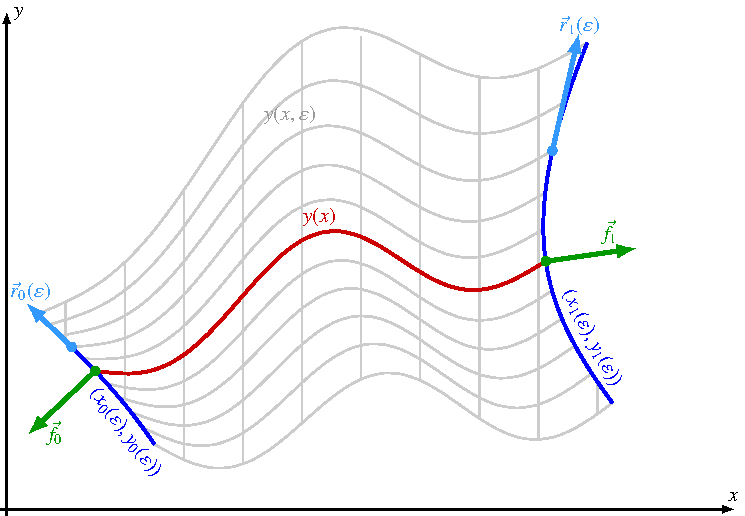
\includegraphics{chapters/020-variation/images/variation.pdf}
\caption{Bei der allgemeinen Variation einer Funktion $y(x)$
varieren sowohl die $x$- wie auch die $y$-Werte der Endpunkte
der Kurve
$x\colon [x_0(\varepsilon),x_1(\varepsilon)]\to\mathbb{R}
:
x\mapsto y(x,\varepsilon)$.
\label{buch:variation:fig:variation}}
\end{figure}
